\documentclass[12pt,letterpaper]{article}
\usepackage[utf8]{inputenc}
\usepackage[spanish]{babel}
\usepackage{amsmath}
\usepackage{amsfonts}
\usepackage{amssymb}
\usepackage{graphicx}
\usepackage{lmodern}
\usepackage{kpfonts}
\usepackage{fourier}
\usepackage{color}
\usepackage{listings}
\usepackage{hyperref}
\usepackage{multicol}
\usepackage{multirow, array}
\usepackage{enumerate}
\usepackage[left=2.5cm,right=2cm,top=2cm,bottom=2cm]{geometry}
\usepackage{float}
\usepackage{fancyhdr}
\usepackage{quotchap}
\usepackage{tikz}
\usepackage[hidelinks]{hyperref}
\usepackage{chemfig}
\usepackage{pgfplots}
\usepackage{booktabs}
%\usepackage{color}      % Definición de colores
%    \hypersetup{colorlinks=true, linkcolor=[rgb]{0,0,1}, citecolor=[rgb]{0,0,1}}
\usepackage{xcolor}		% Permite definir un color para utilizarlo dentro del documento.
%    \definecolor{gris}{RGB}{70,70,70}	    % Definiendo el color gris
%    \definecolor{negro}{RGB}{40,40,40}		% Definiendo el color negro

%%%%%%%% Modificación de los espacios de los títulos de secciones %%%%%%%%%%
\usepackage{titlesec}		% Permite reconfigurar  los títulos de las secciones y subsecciones
%% =============================================================================
%%  OTRA COSA QUE NO SEAN PAKETES
%% =============================================================================
\pagestyle{fancy}
\setcounter{secnumdepth}{3}
\setcounter{tocdepth}{4}
\fancyhf{}
\rhead{I5839 D-03}
\lhead{Laboratorio de reactores(2020B)}
\rfoot{\thepage}
%\renewcommand\thesection{\Roman{section}}	% Numeración romana en las secciones
%\renewcommand\thesubsection{\Roman{subsection}}		% Numeración romana en las subsecciones
\titlespacing*{\section}{0pt}{2.5mm}{0mm}	% Espaciado del título {espacio izquierdo}{arriba del título}{abajo del título}
\titleformat{\section}[block]{\large\scshape\centering}{\thesection.}{1em}{}
\titleformat{\subsection}[block]{\large}{\thesubsection.}{1em}{}
%\newcommand{\colorhrule}[3]{\begingroup\color{#1}\rule{#2}{#3}\endgroup}

\setlength{\intextsep}{1mm} % Distancia superior e inferior en objetos flotantes
\setlength{\columnsep}{5mm} % Separación entre columnas del documento
\spanishdecimal{.}
%% =============================================================================
%%    INICIO DEL DOCUMENTO
%% =============================================================================
\begin{document}
\renewcommand{\tablename}{Tabla}
\thispagestyle{empty}
%======================
%       PORTADA
%======================
\sloppy     % Evita que las palabras se corten al saltar de línea.
\begin{center}
  \begin{tabular}{cc}

\multirow{2}{3.5cm}{
\includegraphics[width=3cm]{Figuras/udg.pdf}}	& \huge{\textsc{\textbf{Universidad de Guadalajara}}}\\
 & \scriptsize{\textsc{CENTRO UNIVERSITARIO DE CIENCIAS EXACTAS E INGENIERÍAS}}\\[5mm]
 & \Large{\textsf{\textbf{Práctica 4. Distribución de tiempos de residencia
}}}\\
 & \\ \vspace{5mm}
 & \small{\textsf{Alejandro Leviatán Gallifrey  [213521903]}}\\
 & \small{\textsc{Ingeniería Química $|$  - Laboratorio de reactores Químicos}}\\
 & \today\\
 & \small{\textit{Profersor:}}  \textbf{\small{Alejandro Nava Tellez }}\\
  \end{tabular}
\end{center}

%\begin{center}
 % \colorhrule{negro}{16.5cm}{1.2pt}
%\end{center}

\rule{\linewidth}{0.75mm}

\tableofcontents
    A partir de observaciones experimentales, Arrhenius estableció la dependencia que la
    constante de velocidad específica de una reacción tiene con la temperatura:
            \[k=A exp \left( \frac{-E_{a}}{RT}\right ) \]
    Donde $k$ es la constante de velocidad, $A$ el denominado factor de frecuencia, $E_a$ la
    energía de activación, $R$ la constante de los gases y $T$ la temperatura expresada en
    Kelvin. Si se realizan experimentos a diferentes temperaturas, se pueden determinar
    los parámetros $A$ y $E_a$ a partir de la representación lineal de la ecuación de Arrhenius
    en su forma logarítmica:
            $$ ln k =ln A - \dfrac{E_a}{R} \dfrac{1}{T} $$
%
%
%
\section{Objetivos}

Analizar el efecto de la temperatura y determinar los parámetros de la ecuación de
Arrhenius: energía de activación y factor de frecuencia.
\section{Prerreporte}
    \begin{enumerate}
        \item ¿Cuáles son las características de una reacción exotérmica y de una endotérmica?
            \begin{itemize}
                \item Exotérmica:
            \end{itemize}
        Durante una reacción exotérmica el calor \textit{sale} o fluye \textit{hacia afuera} del sistema, es decir, hacia el entorno.

                $$\Delta H<0$$

            \begin{itemize}
                \item Endotérmica:
            \end{itemize}
        Durante una reacción endotérmica, el calor fluye \textit{hacia dentro} 
        del sistema desde su entorno.

                $$\Delta H>0$$

        \item Que representan el factor de frecuencia y la enería de activación.
            \begin{itemize}
                \item Factor de frecuencia:
            \end{itemize}
        El factor de frecuencia "\textit{A}" es una relación empírica entre la
        temperatura y el coeficiente de velocidad.

            \begin{itemize}
                \item Energía de activación:
            \end{itemize}

         Es la energía mínima que necesita un sistema antes de poder iniciar la
          reacción.

        \item  ¿Cuál es el efecto de la temperatura en una reacción química?

        La temperatura influye directamente en la velocidad de reacción. Mientras mayor
        sea la temperatura mayor es el número de choques entre las moléculas y mayor 
        la velocidad de la reacción.
    \end{enumerate} 
    
    \subsection{Materiales y reactivos}
    
    Para el desarrollo de esta práctica se requiere un reactor esférico con 3 bocas esmeri-
    ladas de 250 mL, un soporte universal, una pinza de 3 dedos, dos tapones de hule, 
    un condensador, manguera, un cronómetro y dos probetas de 100 mL, 2 vasos de 
    precipitados de 100 mL, una propipeta, un conductímetro, una pizeta, dos matraces 
    aforados de 100 mL, una espátula, un termómetro, un agitador magnético y una barra 
    de agitación magnética. Además se requieren 100 mL de una solución de 0.2 M de NaOH 
    y 100 mL de una solución 0.2 M de acetato de etilo. Y también se necesita



    \subsection{Procedimiento}
    
    Preparar las soluciones de NaOH y de acetato de etilo. En el reactor perfectamente
    limpio y seco, colocar 100 mL de solución de $NaOH$ $0.2\: M $. Fijar el reactor al soporte
    universal e introducir en el baño térmico ajustando la temperatura de reacción. Medir
    con la probeta 100 mL de acetato de etilo y vaciarlos a un vaso de precipitados. Colocar
    el termómetro y el conductimetro en el reactor. Vaciar la solución medida de acetato
    de etilo al reactor, agitar vigorosamente durante unos segundos con ayuda del agitador
    magnético y poner en marcha el cronómetro. Hacer medidas de conductividad para la
    reacción a los siguientes tiempos: 0.5, 1, 1.5, 2, 3, 5, 7, 10, 13 y 18. Una vez realizadas
    las mediciones anteriores, vaciar la muestra en un frasco de vidrio, cierre y deje enfriar
    a temperatura ambiente. Este procedimiento se deberá realizar para las siguientes
    temperaturas: 35, 50, 65 y 80 $^{\circ}$C. Deberán obtenerse las curvas de calibración a cada
    temperatura.

    \subsection{Diagrama}
        \begin{figure}[H]
            \centering
            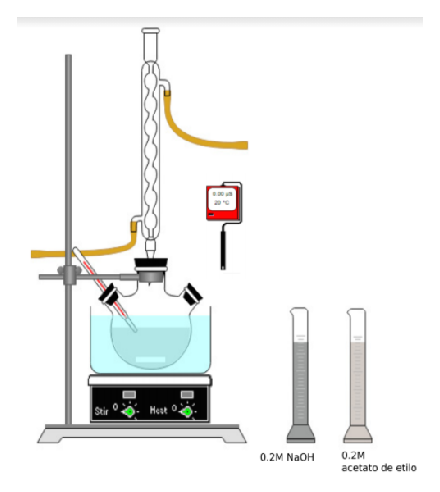
\includegraphics[scale=0.7]{Figuras/Diagrama.eps}
            \caption{Diagrama de la práctica}
        \end{figure}

\section{Cálculos}


\begin{enumerate}
        \item Expresar la ley de velocidad para la reacción.
         Para este caso $ A$ es acetato de etilo y $B$ es el Hidróxido de sodio.

                $$ -r_{a}= k[A][B] $$
        \item Elaborar una gráfica de conductividad en función del tiempo y 
        extrapolar a t = 0.

     \begin{figure}[H]
         \centering
         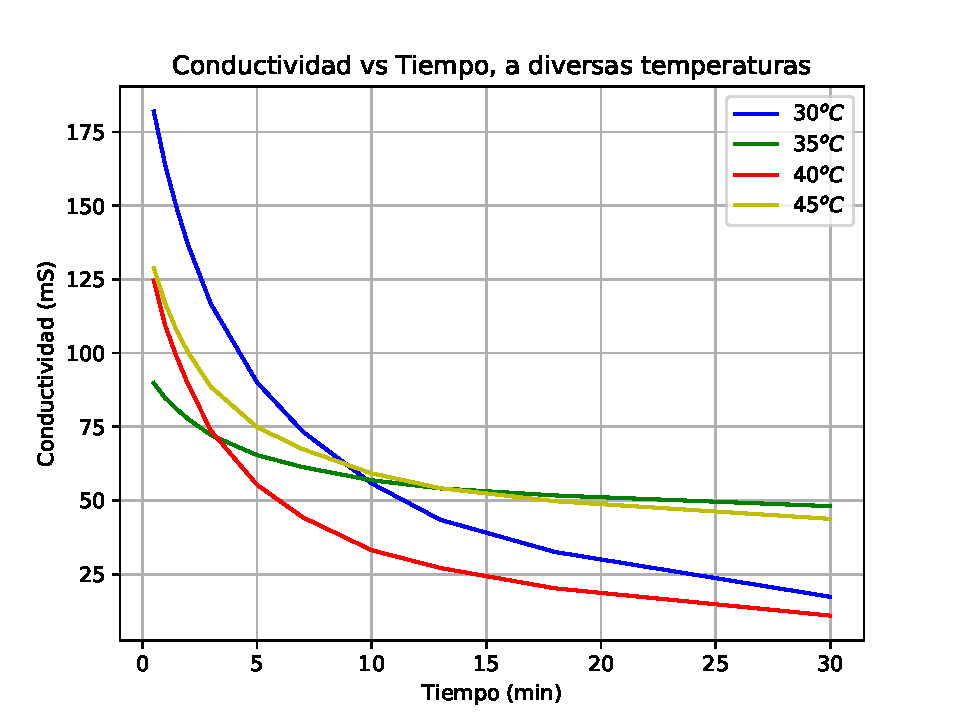
\includegraphics[scale = 0.8]{Figuras/Conductividad_vs_Tiempo.pdf}
         \caption{Diagrama de la pr\'{a}ctica}
      \end{figure}

      \item Plantear las ecuaciones de conductividad en función del tiempo.
       A partir de estas ecuaciones, determinar las concentraciones de los productos 
       que se han formado a cualquier tiempo t, en función de la conductividad.\\
      Con los siguientes  datos se elabora una gráfica de calibración para obtener 
      las concentraciones a cualquier tiempo.

% Table generated by Excel2LaTeX from sheet 'Hoja1'
\begin{table}[H]
  \centering
  \caption{Datos de la práctica}
    \begin{tabular}{crrrr}
    \hline
    \multicolumn{1}{l}{Temperatura} & $30 \: C^{ \circ}$    & $35\: C^{ \circ}$    & $40\: C^{ \circ}$    & $45\: C^{ \circ}$ \\
    \multicolumn{1}{c}{\multirow{2}[0]{*}{Tiempo}} & \multicolumn{1}{p{4.335em}}{Conducti} & \multicolumn{1}{p{4.445em}}{Conducti} & \multicolumn{1}{p{4.28em}}{Conducti} & \multicolumn{1}{p{3.945em}}{Conducti} \\
          & \multicolumn{1}{p{4.335em}}{vidad(mS)} & \multicolumn{1}{p{4.445em}}{vidad(mS)} & \multicolumn{1}{p{4.28em}}{vidad(mS)} & \multicolumn{1}{p{3.945em}}{vidad(mS)} \\ \hline
    0.5   & 181.95 & 89.82 & 124.65 & 128.8 \\
    1     & 163.65 & 84.74 & 109.24 & 116.77 \\
    1.5   & 149.17 & 80.97 & 98.64 & 107.59 \\
    2     & 136.56 & 77.64 & 89.3  & 100.18 \\
    3     & 116.54 & 72.14 & 73.6  & 88.49 \\
    5     & 90.12 & 65.4  & 55.33 & 74.91 \\
    7     & 73.36 & 61.31 & 44.29 & 67.42 \\
    10    & 55.79 & 56.87 & 33.14 & 59.22 \\
    13    & 43.44 & 54.1  & 27.1  & 54.17 \\
    18    & 32.54 & 51.72 & 20.2  & 49.76 \\
    30    & 17.33 & 48.08 & 10.95 & 43.78 \\ \hline
    \end{tabular}%
  \label{tab:addlabel}%
\end{table}%
  

        \begin{figure}[H]
            \centering
            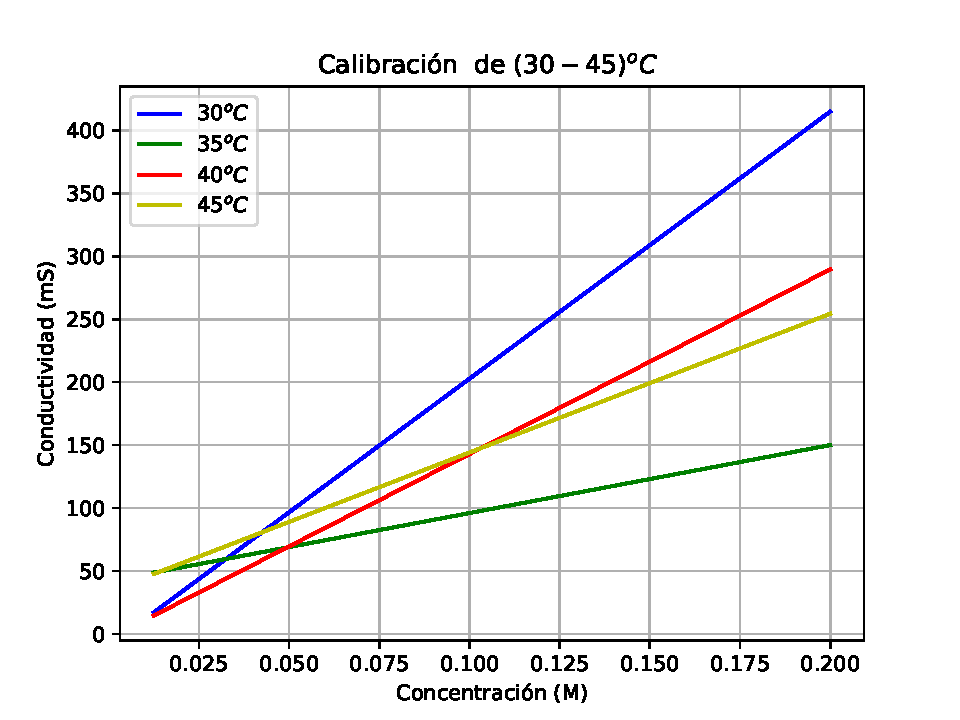
\includegraphics[scale = 0.8]{Figuras/calibracion_todos.pdf}
            \caption{Diagrama de la pr\'{a}ctica}
        \end{figure}

    Con esta gráfica se tiene el ajuste de polinomio:
            $$  Conductividad = m[x] + b$$

        \begin{figure}[H]
            \centering
            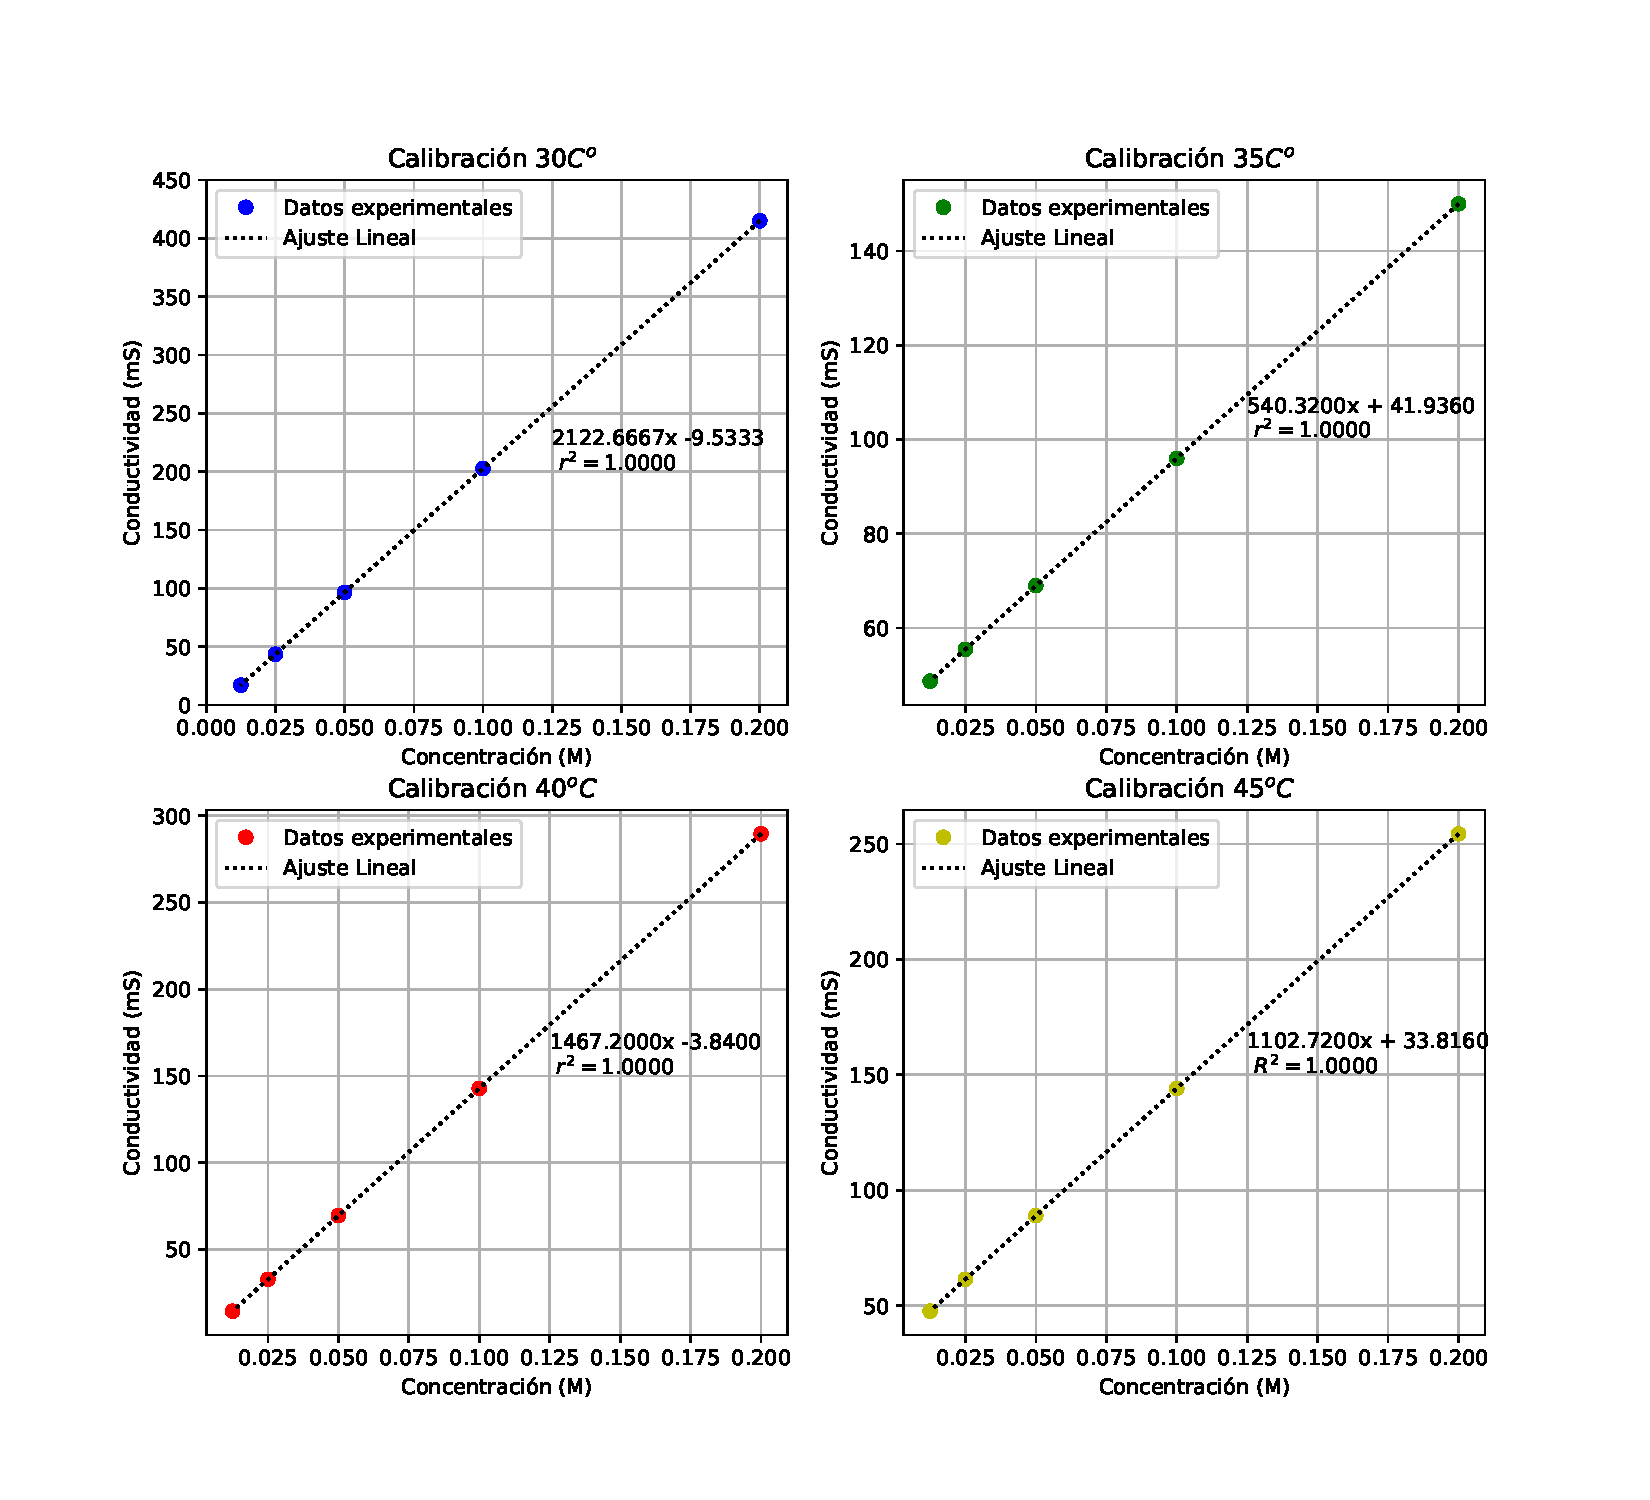
\includegraphics[scale=0.65]{Figuras/FiguraTodos.pdf}
            \caption{Diagrama de la pr\'{a}ctica}
        \end{figure}

\begin{figure}[H]
    \centering
\begin{tabular}{cccc}
\hline
$ T (^{\circ}$C) & Pendiente (m) & Intercepto & $r^{2}$ \\
\hline
30 & 2122.7 & -9.5334  & 1   \\
35 & 540.32 & +41.936  & 1   \\
40 & 1467.2 & -3.84    & 1   \\
45 & 1102.7 & +33.813  & 1   \\
\hline

\end{tabular} 
\caption{Datos  de calibración }
    \label{fig:my_label}
\end{figure}


    Despejando para la concentración tenemos que:
            $$ [x]= \dfrac{Conductividad + b}{m}$$
            
    Se calculan las concentraciones siguientes:\\

\begin{table}[H]
    \centering
    \begin{tabular}{crrrr}
        \hline
        
        \multicolumn{1}{l}{Temperatura} & $30 C^{\circ} $   & $35 \: C^{\circ}$    & $40 \: C^{\circ}$    & $45 \: C^{\circ}$ \\ \hline
        \multicolumn{1}{c}{\multirow{2}[0]{*}{Tiempo}} & \multicolumn{1}{p{5.39em}}{Concen-} & \multicolumn{1}{p{5.39em}}{Concen-} & \multicolumn{1}{p{5.39em}}{Concen-} & \multicolumn{1}{p{5.39em}}{Concen-} \\ 
              & \multicolumn{1}{p{5.39em}}{tración (M)} & \multicolumn{1}{p{5.39em}}{tración (M)} & \multicolumn{1}{p{5.39em}}{tración (M)} & \multicolumn{1}{p{5.39em}}{tración (M)} \\ \hline
        0.5   & 0.09021 & 0.08862 & 0.08757 & 0.08614 \\
        1     & 0.08159 & 0.07922 & 0.07707 & 0.07523 \\
        1.5   & 0.07476 & 0.07224 & 0.06985 & 0.0669  \\
        2     & 0.06882 & 0.06608 & 0.06348 & 0.06018 \\
        3     & 0.05939 & 0.0559  & 0.05278 & 0.04958 \\
        5     & 0.04695 & 0.04343 & 0.04033 & 0.03727 \\
        7     & 0.03905 & 0.03586 & 0.0328  & 0.03047 \\
        10    & 0.03077 & 0.02764 & 0.0252  & 0.02304 \\
        13    & 0.02496 & 0.02251 & 0.02109 & 0.01846 \\
        18    & 0.01982 & 0.01811 & 0.01638 & 0.01446 \\
        30    & 0.01266 & 0.01137 & 0.01008 & 0.00904 \\ 
        
        \hline
    \end{tabular}
    \caption{Tabla de concentraciones a diferentes temperaturas}
    \label{tab:concentracion}
\end{table}
  

    \item Utilizando las concentraciones anteriormente calculadas, determinar el orden de
    reacción y la constante de velocidad por el método integral gráfico.\\
    Para calcular el orden de reacción se gráfica $t$ vs $1/C_a$\\

\begin{table}[H]
    \centering
    \begin{tabular}{crrrr}
        \hline

        \multicolumn{1}{l}{Temperatura} & $30\: ^{\circ} C$    & $35\: ^{\circ} C$    & $40\: ^{\circ} C$    & $45\: ^{\circ} C$ \\ \hline 
        \multicolumn{1}{c}{\multirow{2}[0]{*}{Tiempo}} & \multicolumn{1}{p{4.5em}}{$1/Ca$} & \multicolumn{1}{p{5.78em}}{$1/Ca$} & \multicolumn{1}{p{6em}}{$1/Ca$} & \multicolumn{1}{p{5.39em}}{$1/Ca$} \\ 
              &       &       &       &  \\ \hline
        0.5   & 11.08556 & 11.28394 & 11.41879 & 11.60932 \\
        1     & 12.25695 & 12.62312 & 12.97489 & 13.29291 \\
        1.5   & 13.37526 & 13.84229 & 14.31694 & 14.94700 \\
        2     & 14.52975 & 15.13332 & 15.75263 & 16.61594 \\
        3     & 16.83702 & 17.88902 & 18.94628 & 20.16864 \\
        5     & 21.30083 & 23.02762 & 24.79635 & 26.83360 \\
        7     & 25.60759 & 27.88892 & 30.48411 & 32.81455 \\
        10    & 32.49525 & 36.18053 & 39.67550 & 43.40655 \\
        13    & 40.07105 & 44.4196  & 47.42081 & 54.17608 \\
        18    & 50.4523  & 55.22486 & 61.03161 & 69.16081 \\
        30    & 79.01829 & 87.94271 & 99.20216 & 110.6684 \\ 
        \hline
        
        \end{tabular}
    \caption{Inversa de la concentración a las diferentes temperaturas}
    \label{tab:inversa_concentracion}
  \end{table}%
  

    \begin{figure}[H]
        \centering
        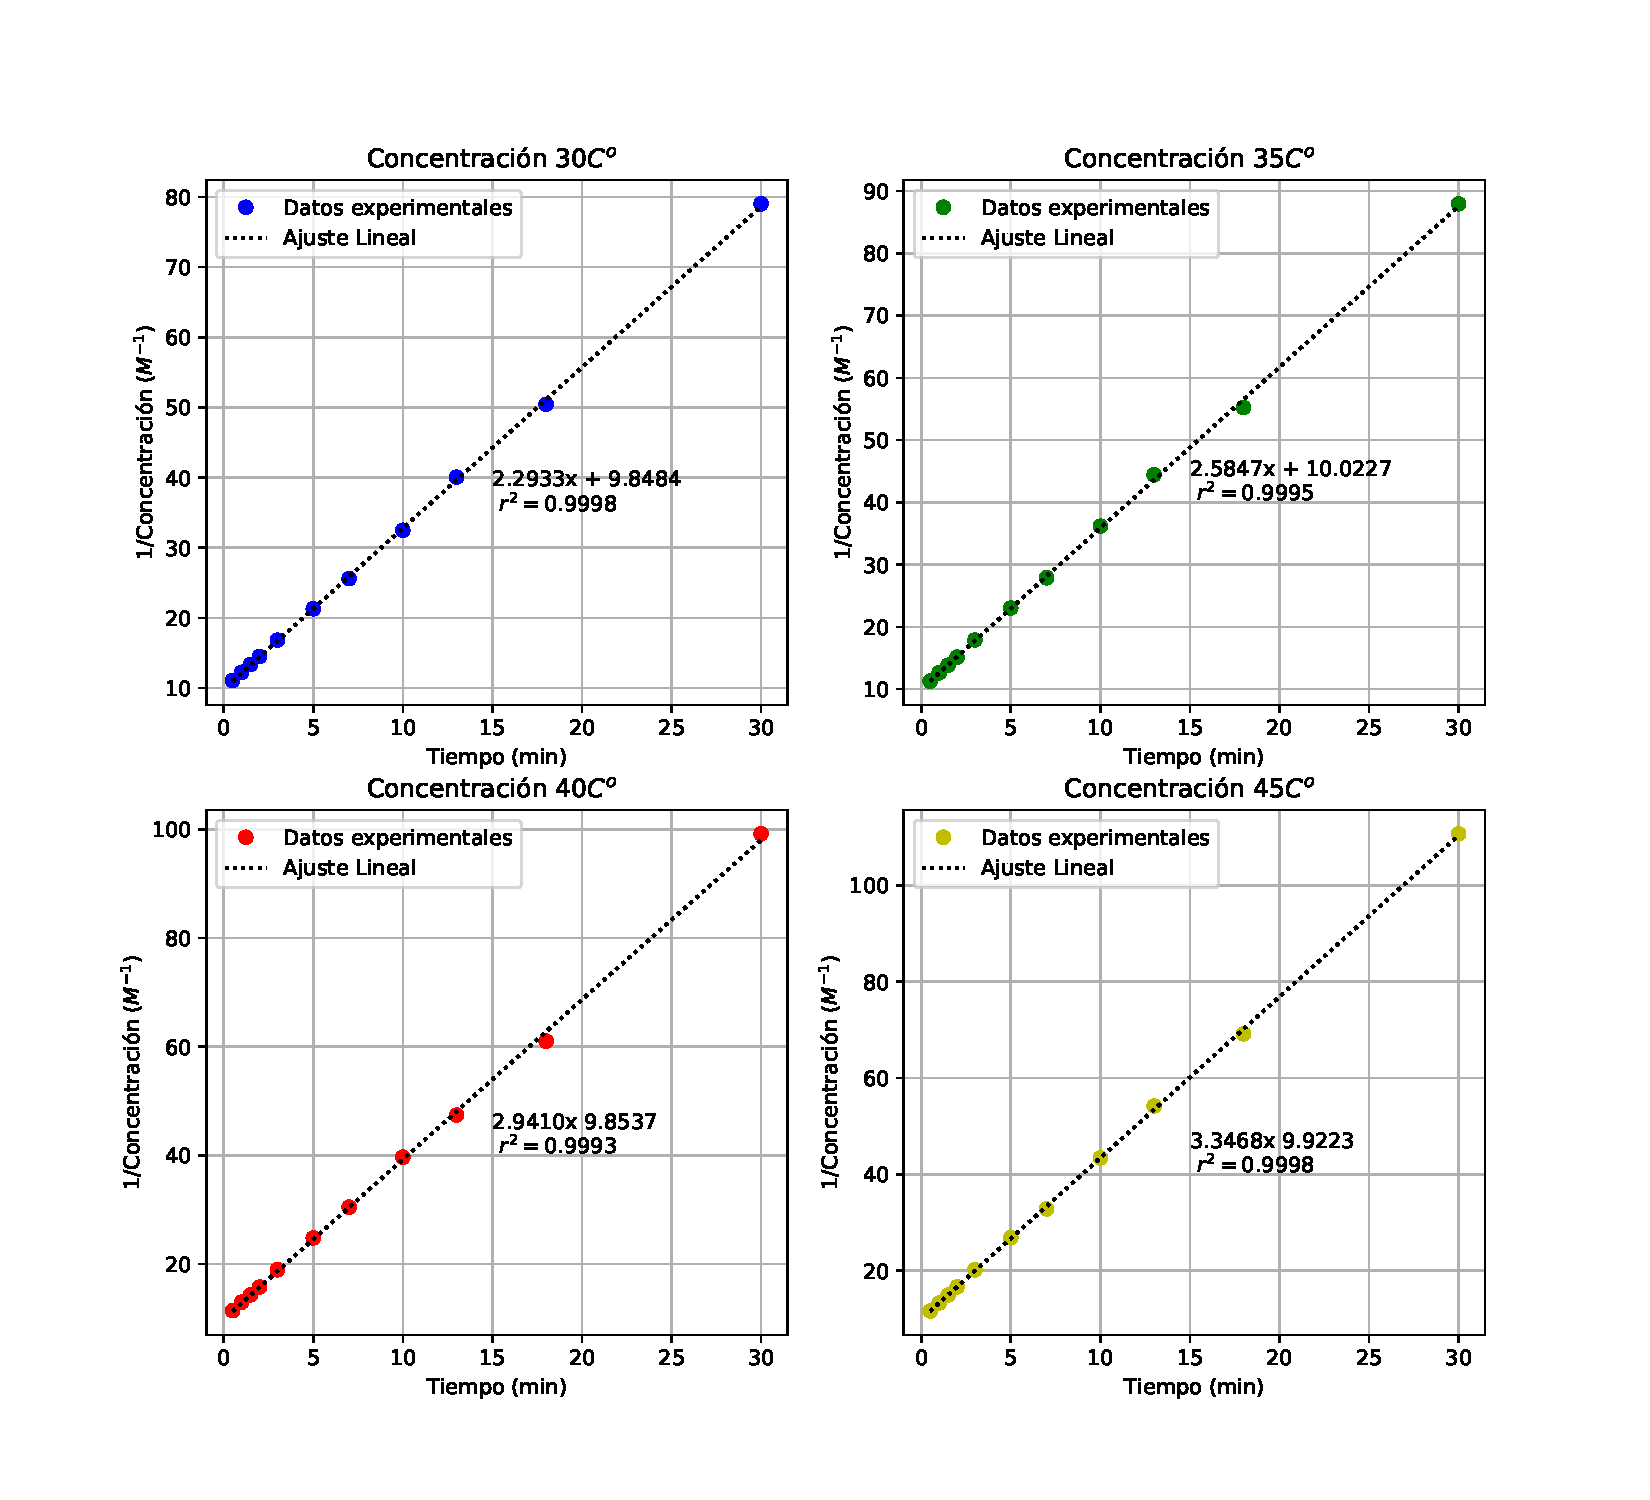
\includegraphics[scale=0.65]{Figuras/Ctodos.pdf}
        \caption{Diagrama de la pr\'{a}ctica}
    \end{figure}

    \begin{figure}[H]
        \centering
        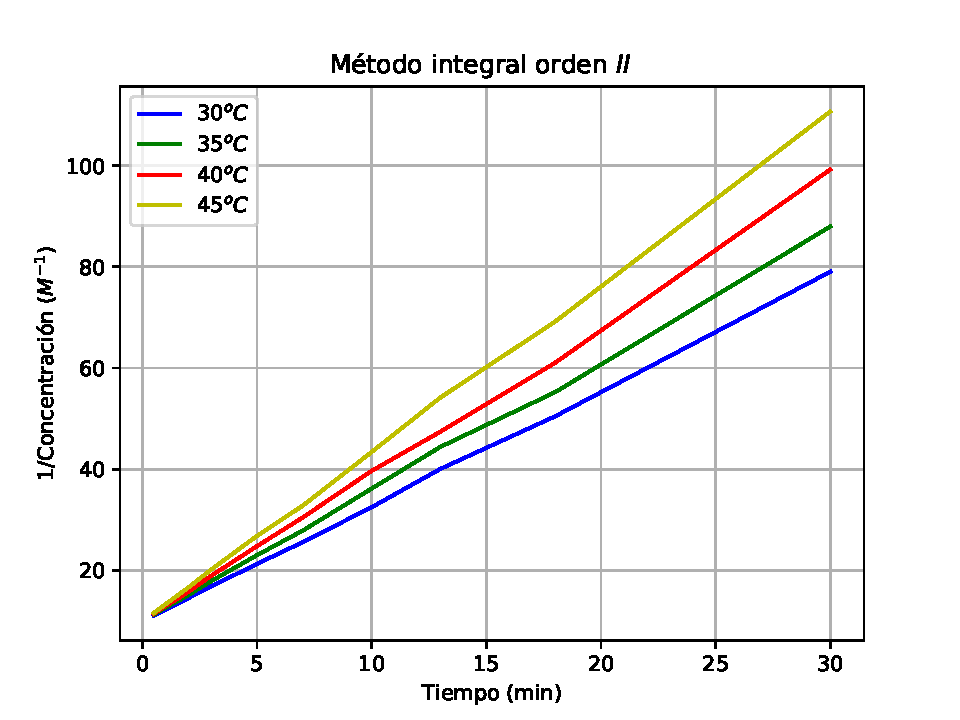
\includegraphics[scale = 0.8]{Figuras/concentracion_todos.pdf}
        \caption{Diagrama de la pr\'{a}ctica}
    \end{figure}



\begin{figure}[H]
    \centering
    \begin{tabular}{cccc}
    \hline
    $ T (^{\circ}$C) & Pendiente(m)=$k$  & Intercepto & $r^{2}$ \\
    \hline
    30 & 2.2934 & 9.8485   & 0.9998  \\
    35 & 2.5847 & 10.023   & 0.9995   \\
    40 & 2.9410 & 9.8537   & 0.9993   \\
    45 & 3.3467 & 9.9221   & 0.9998   \\
    \hline

    \end{tabular} 
\caption{Constantes a diferentes $T$}
    \label{fig:my_label}
\end{figure}\\

    Recordemos que la pendiente  es la contante cinética $ k $, por  el valor de $ r^{2}$  podemos decir que la reacción es de \textbf{orden II}
    \item Calcular el factor de frecuencia (A) y la energía de activación (Ea).\\
    Para calcular los parámetros es necesario tomar las constantes y las temperaturas
    anteriores, aplicando $ln(k)$   y la inversa de la temperatura. Se obtuvo los 
    siguientes datos:\\

\begin{figure}[H]
    \centering
    \begin{tabular}{cccc}
    \hline
    $T$ K & $k$  & $1/T$ & $Ln(k)$ \\
    \hline
    303	& 2.2934 &	0.0033	& 0.8300 \\
    308	& 2.5847 &	0.0032	& 0.9496 \\
    313	& 2.9410 &	0.0032	& 1.0787 \\
    318	& 3.3467 &	0.0031	& 1.2080 \\

    \hline

    \end{tabular} 
\caption{Datos para ecuación de Arrhenius}
    \label{fig:my_label}
\end{figure}\\

Para determinar el parámetro $A$  tenemos que el intercepto $b= 8.8544 = ln(A) $ , despejando tenemos que $A= 7005.144$. Para determinar la energia de activación tenemos que $m= -E_{a}/R$
despejando  tenemos que $E_{a}= 20227.030 J/mol*K$

    \begin{figure}[H]
        \centering
        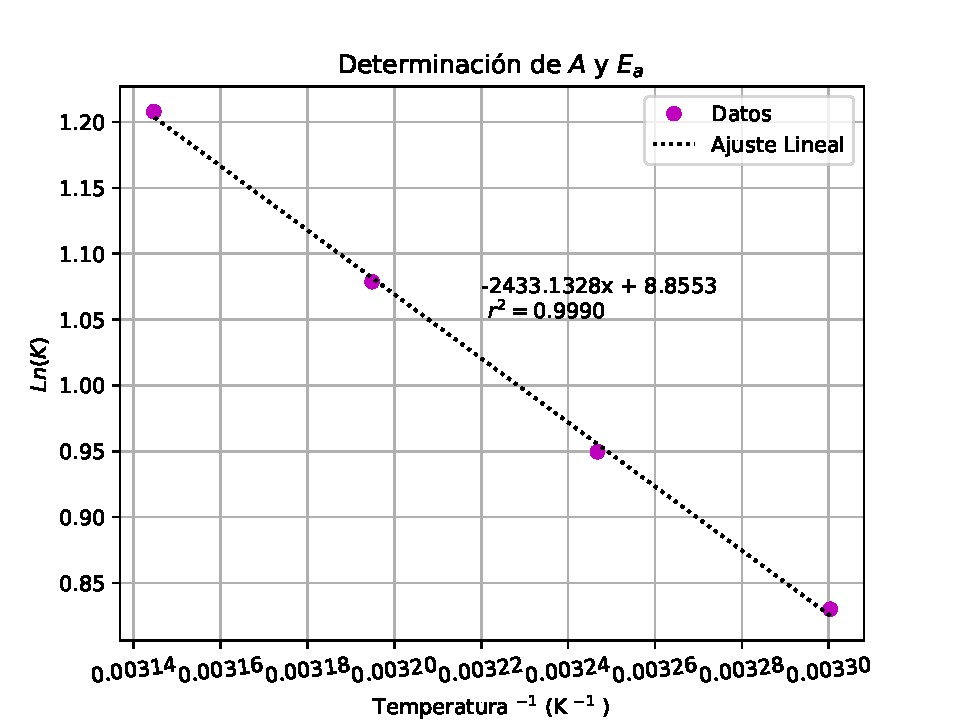
\includegraphics[scale = 0.8]{Figuras/ln_k_t.pdf}
        \caption{Diagrama de la pr\'{a}ctica}
    \end{figure}


\end{enumerate}

\section{Conclusión}

Se calcularon y obtuvieron los parámetros \textit{A} y \textit{$E_{a}$} para la
 ecuación de Arrhenius. En base a la experimentación y los calculos realizados, 
 se concluyo que el aumento de la temperatura afecto directamente la constante 
 cínetica, esto se hizo evidente en la figura 9, donde se observo que al incrementar
  la temperatura los valores de k crecieron ligeramente. 


    



%begin{figure}[H]
%         \centering
%         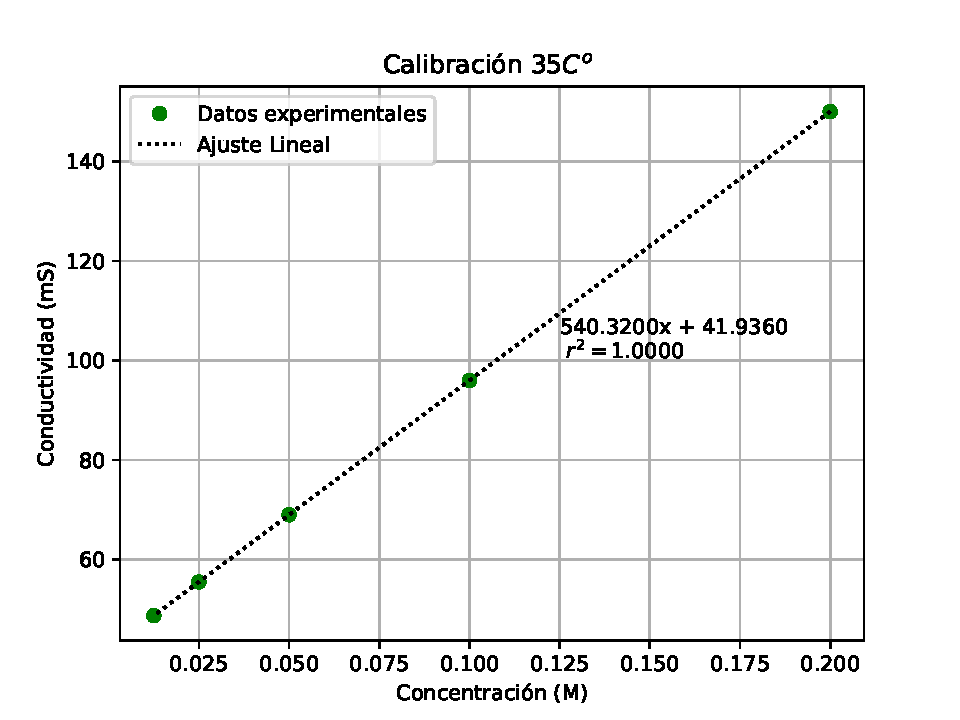
\includegraphics[scale=1]{Figuras/calibracion_35.pdf}
%#         \caption{Diagrama de la pr\'{a}ctica}
%#\end{figure}


%\begin{figure}[H]
%         \centering
%         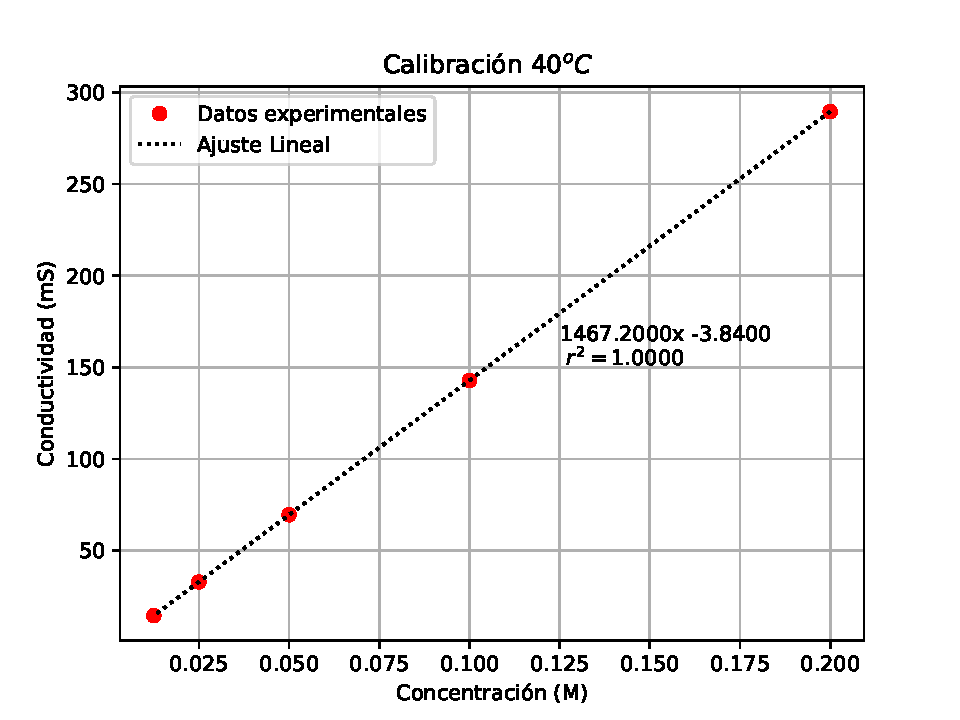
\includegraphics[scale=1]{Figuras/calibracion_40.pdf}
%         \caption{Diagrama de la pr\'{a}ctica}
%\end{figure}



%\begin{figure}[H]
%         \centering
%         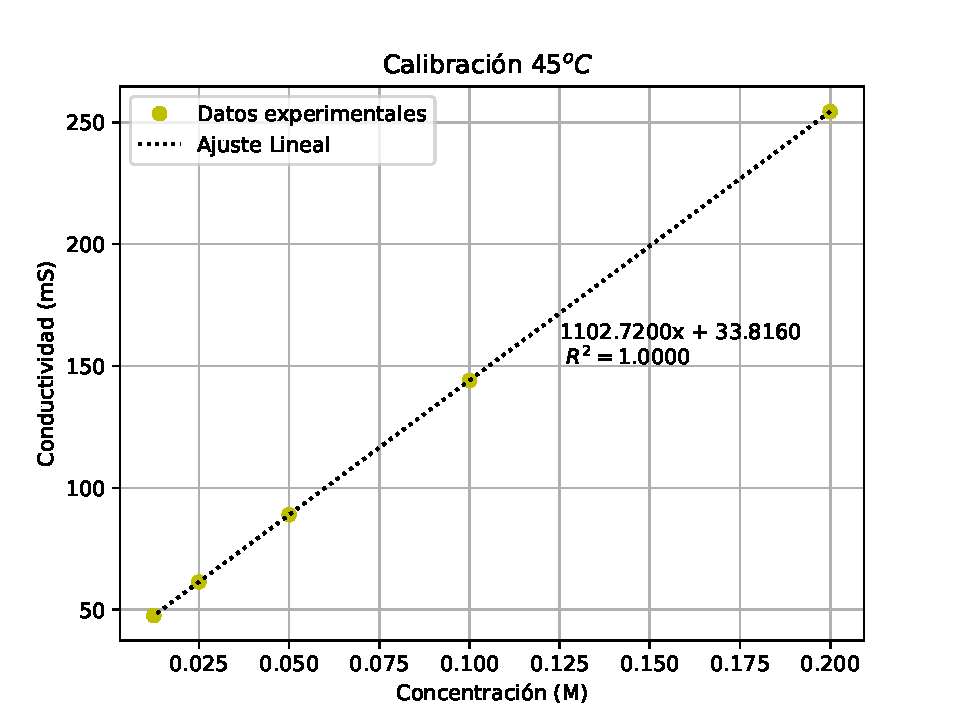
\includegraphics[scale=1]{Figuras/calibracion_45.pdf}
%         \caption{Diagrama de la pr\'{a}ctica}
%\end{figure}



%\begin{figure}[H]
%         \centering
%         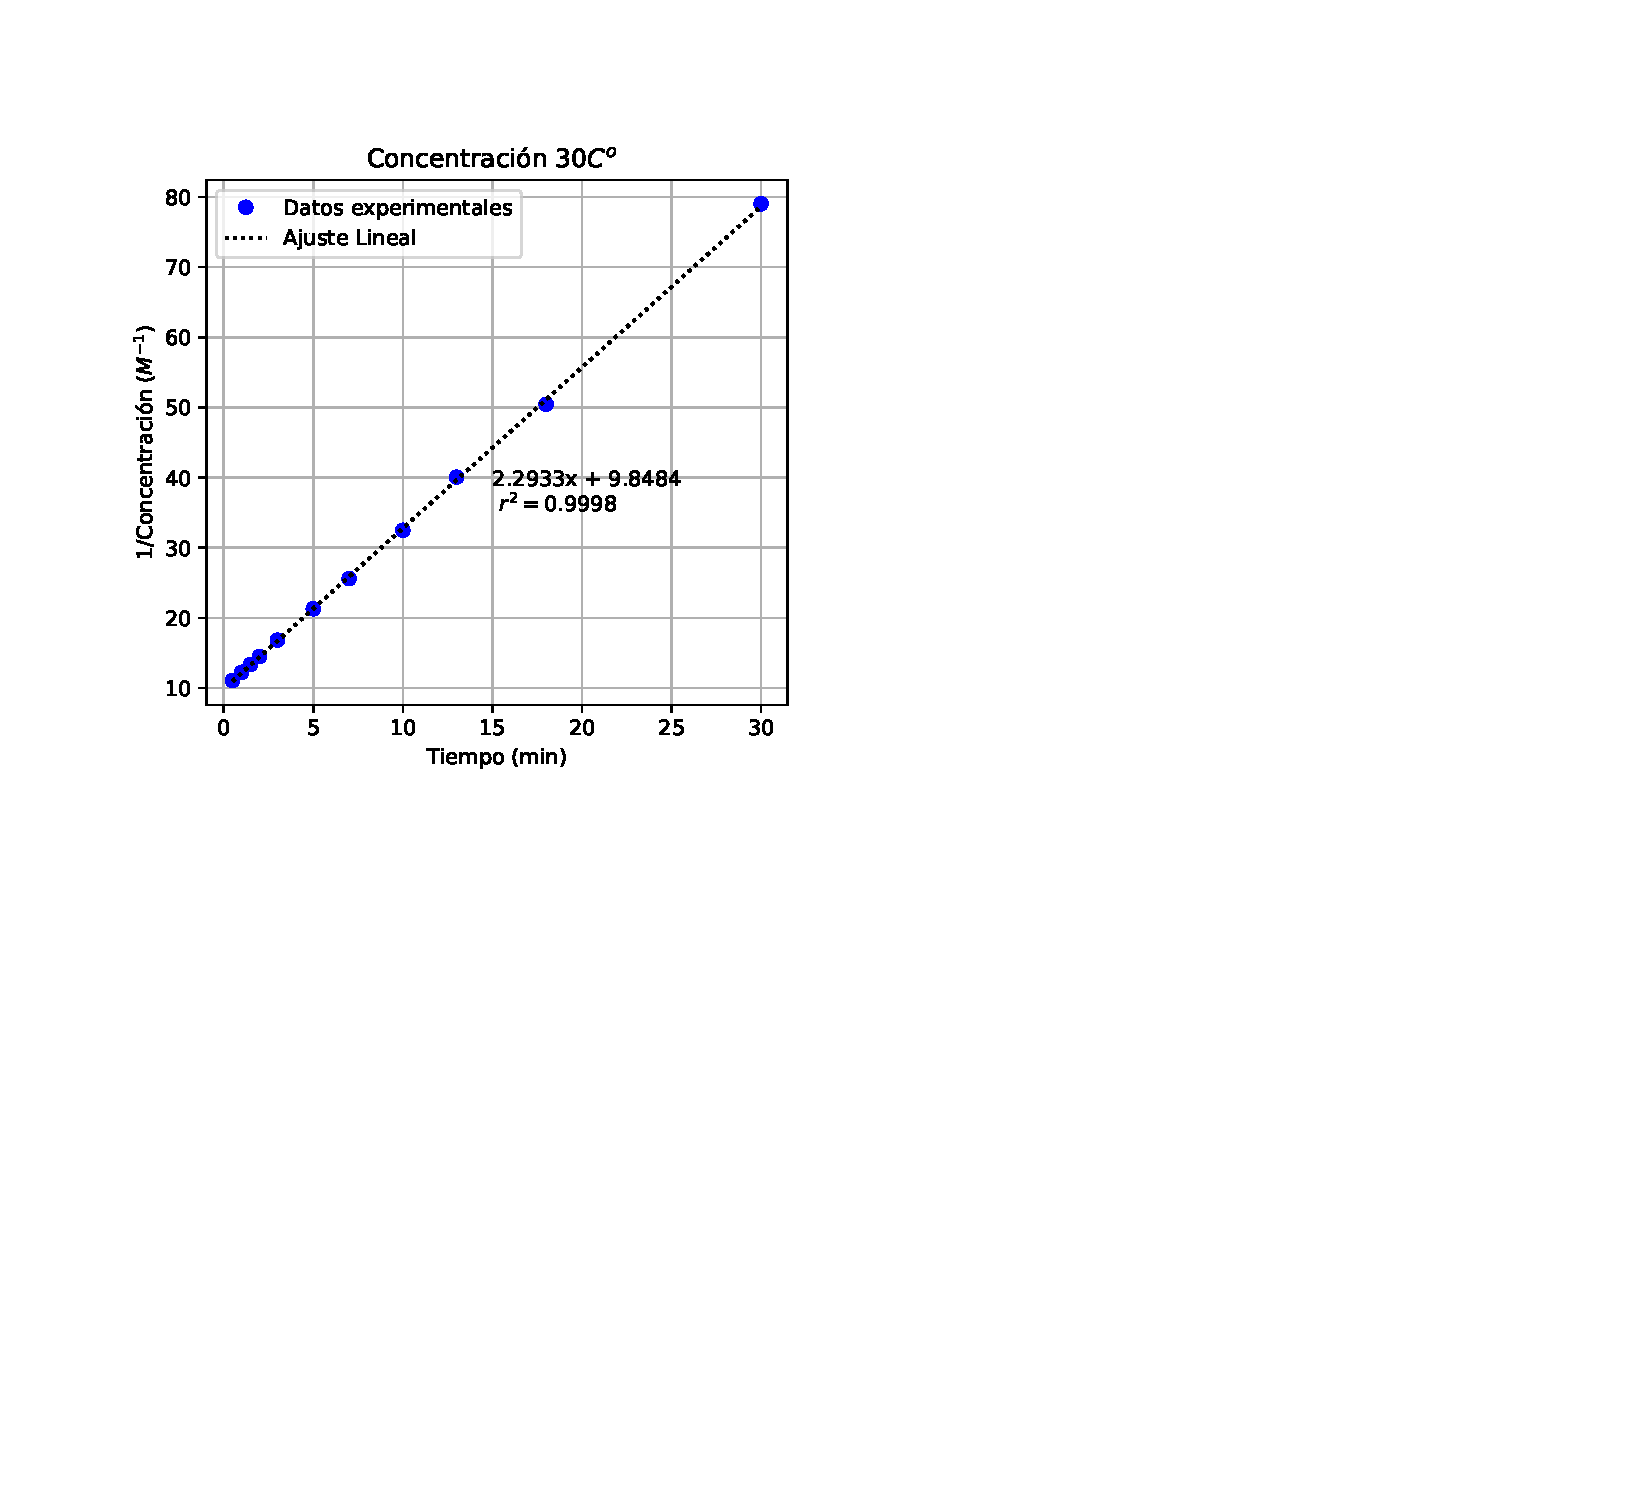
\includegraphics[scale=1]{Figuras/C_30.pdf}
%         \caption{Diagrama de la pr\'{a}ctica}
%\end{figure}


%\begin{figure}[H]
%         \centering
%         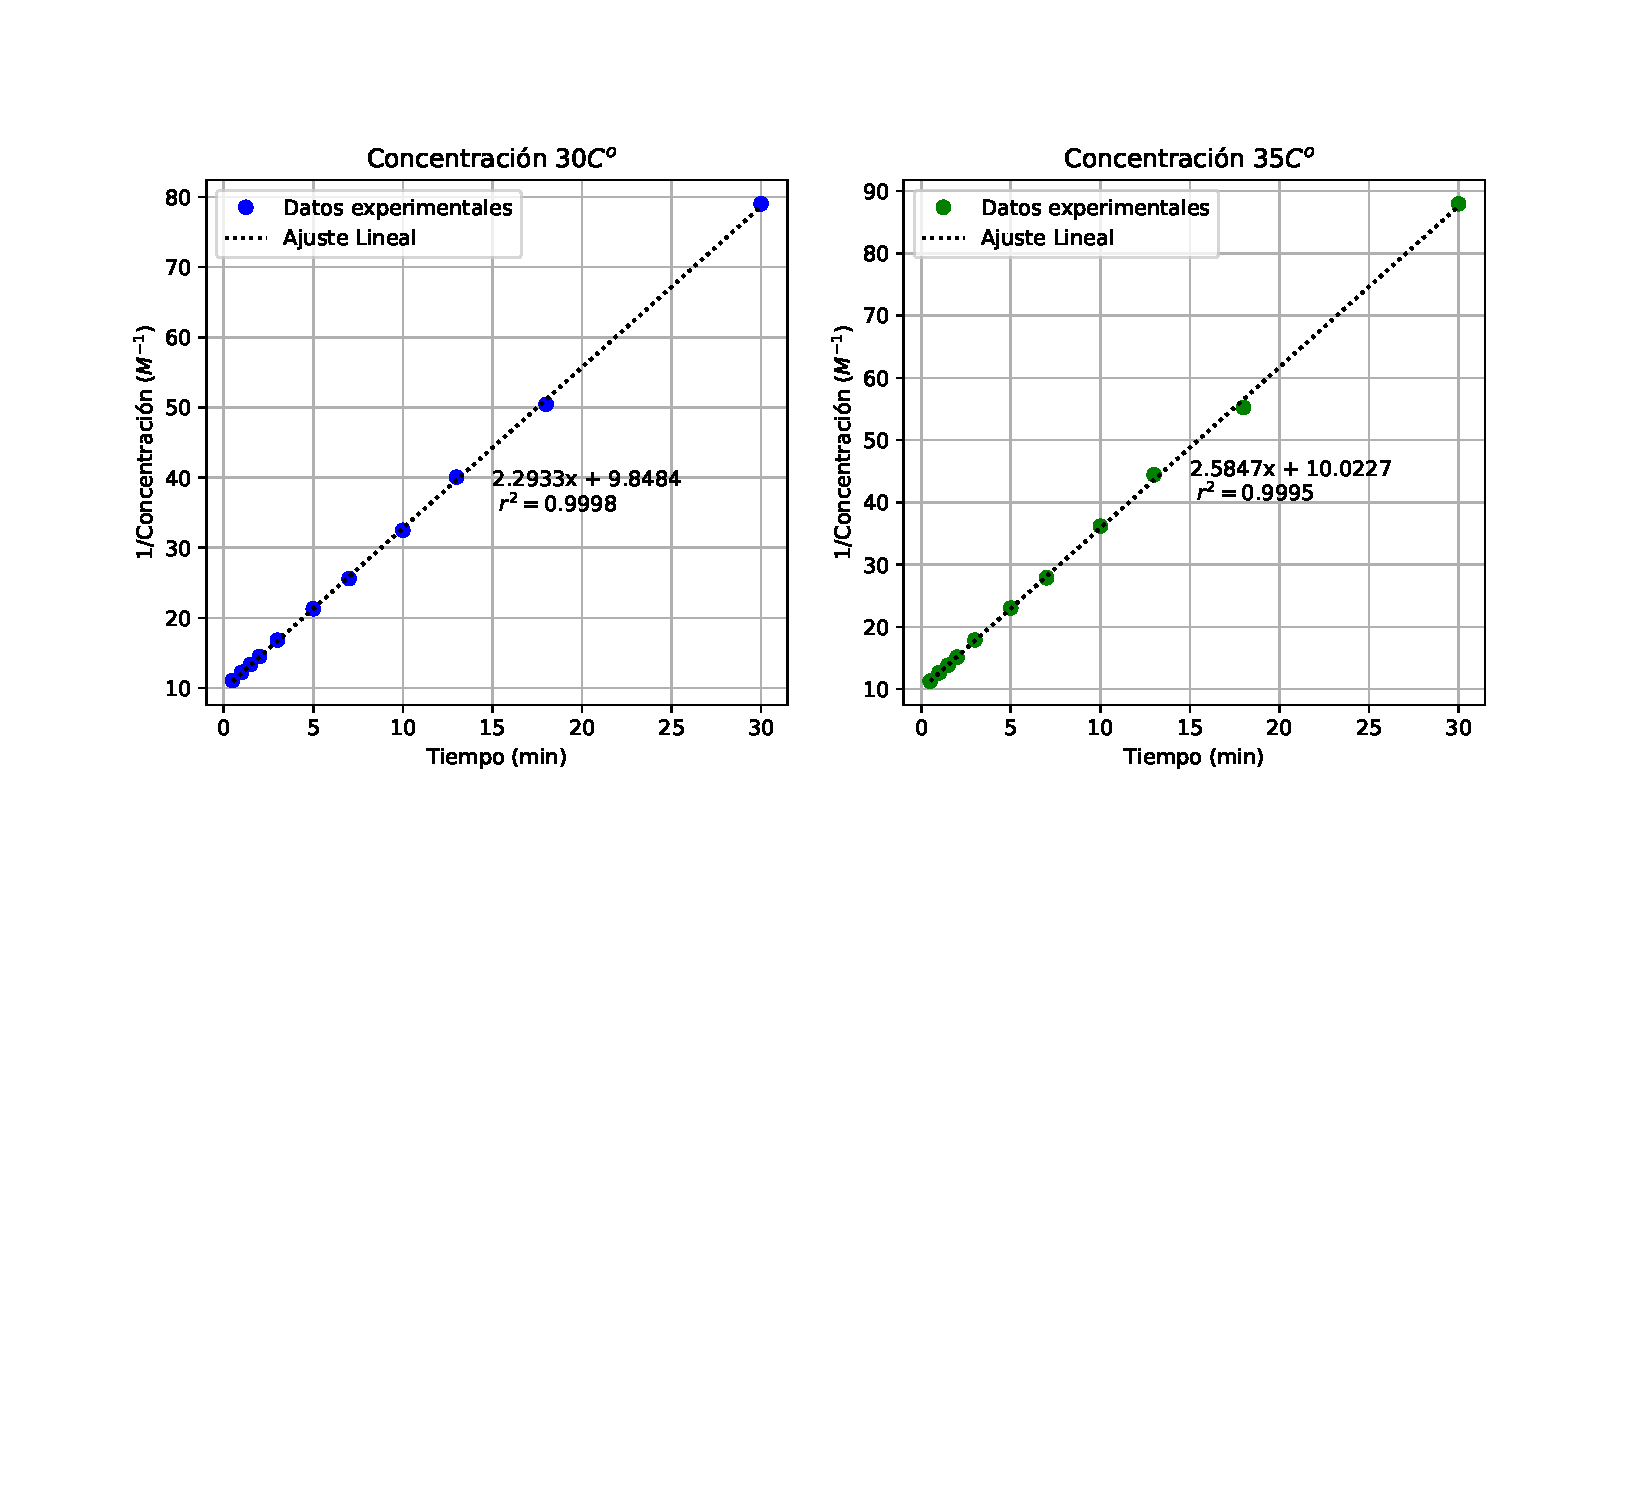
\includegraphics[scale=1]{Figuras/C_35.pdf}
%         \caption{Diagrama de la pr\'{a}ctica}
%\end{figure}


%\begin{figure}[H]
%         \centering
%         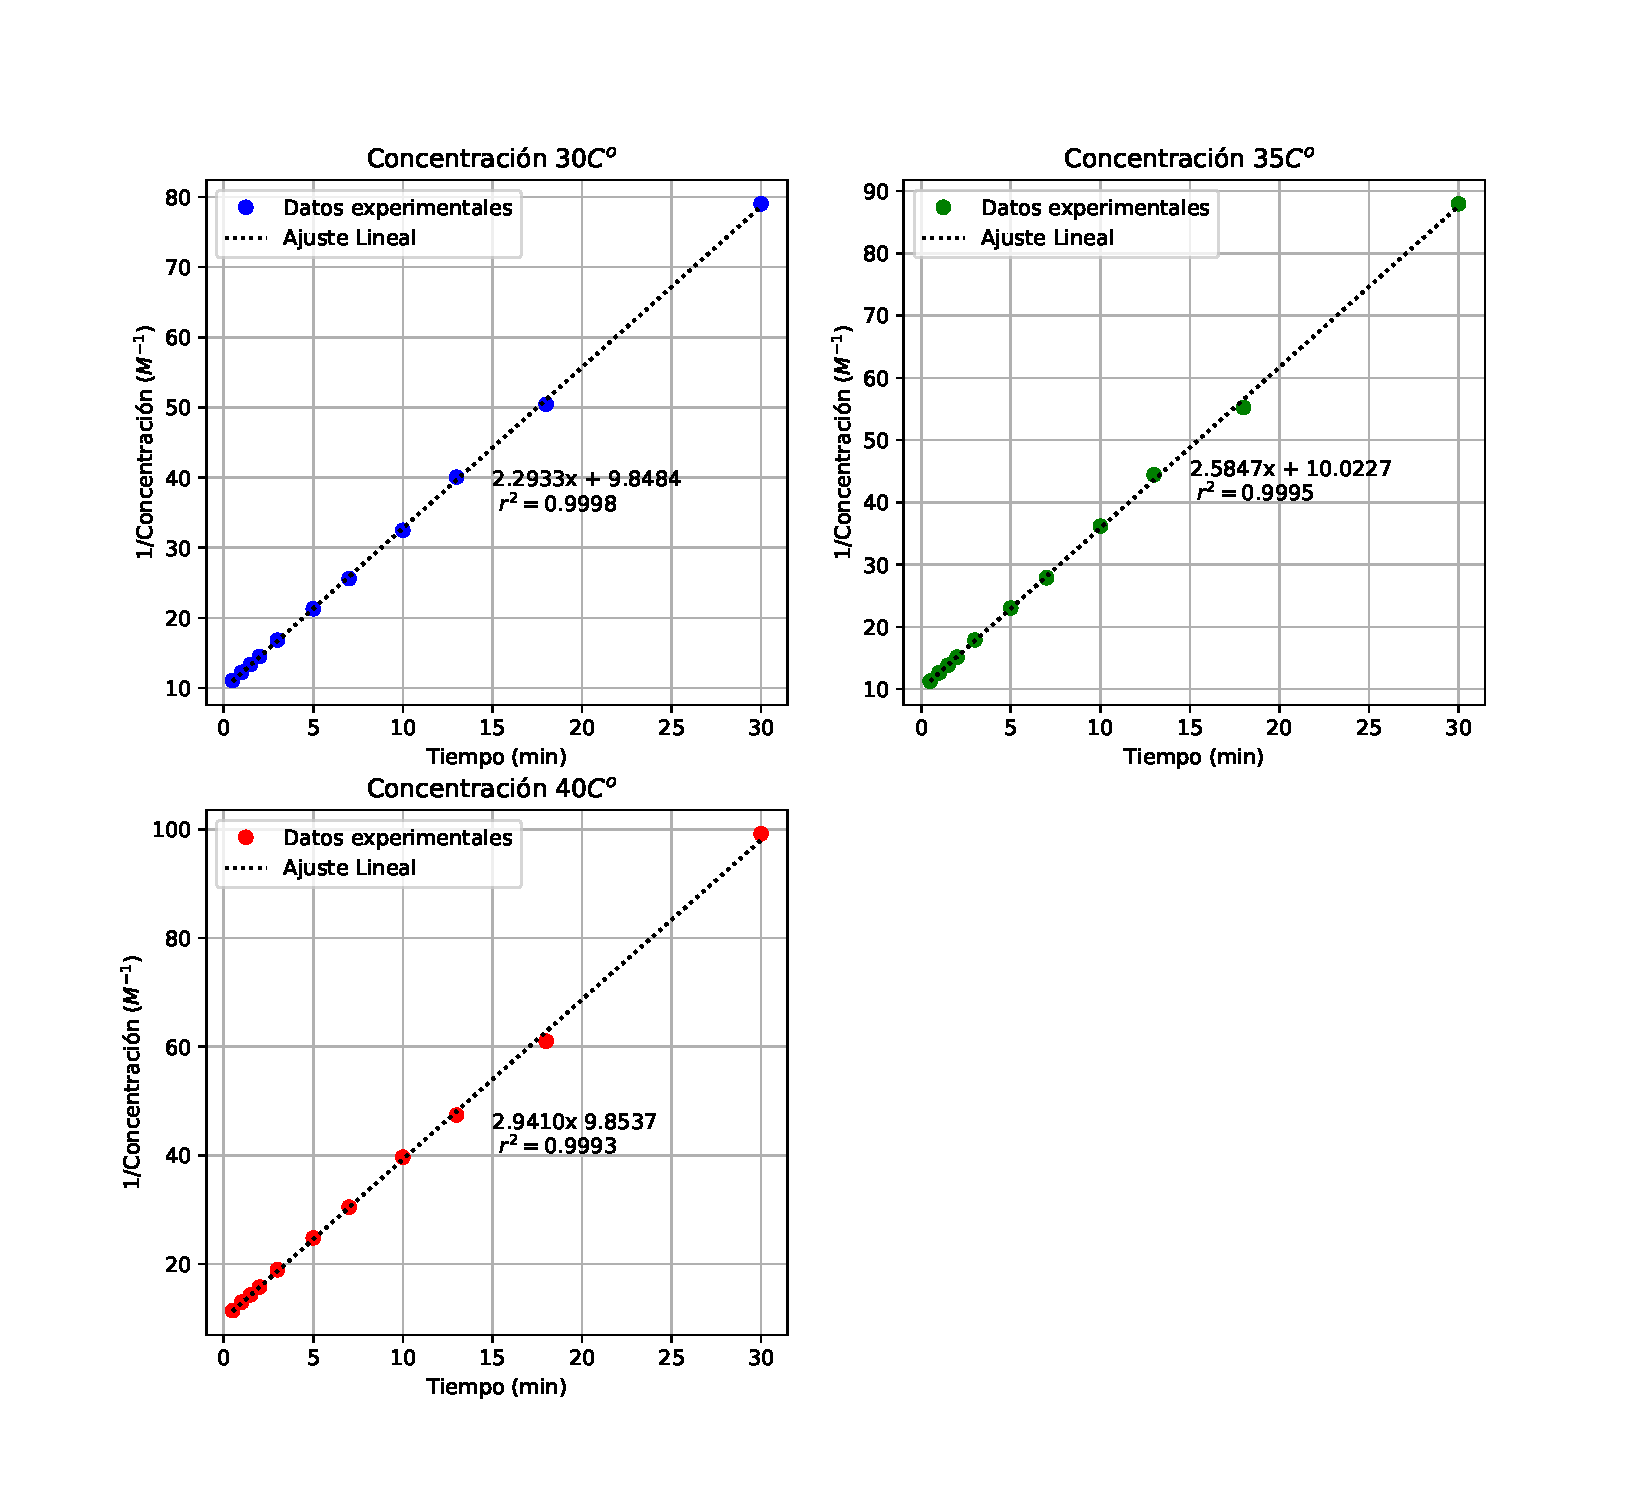
\includegraphics[scale=1]{Figuras/C_40.pdf}
%         \caption{Diagrama de la pr\'{a}ctica}
%\end{figure}


%\begin{figure}[H]
%         \centering
%         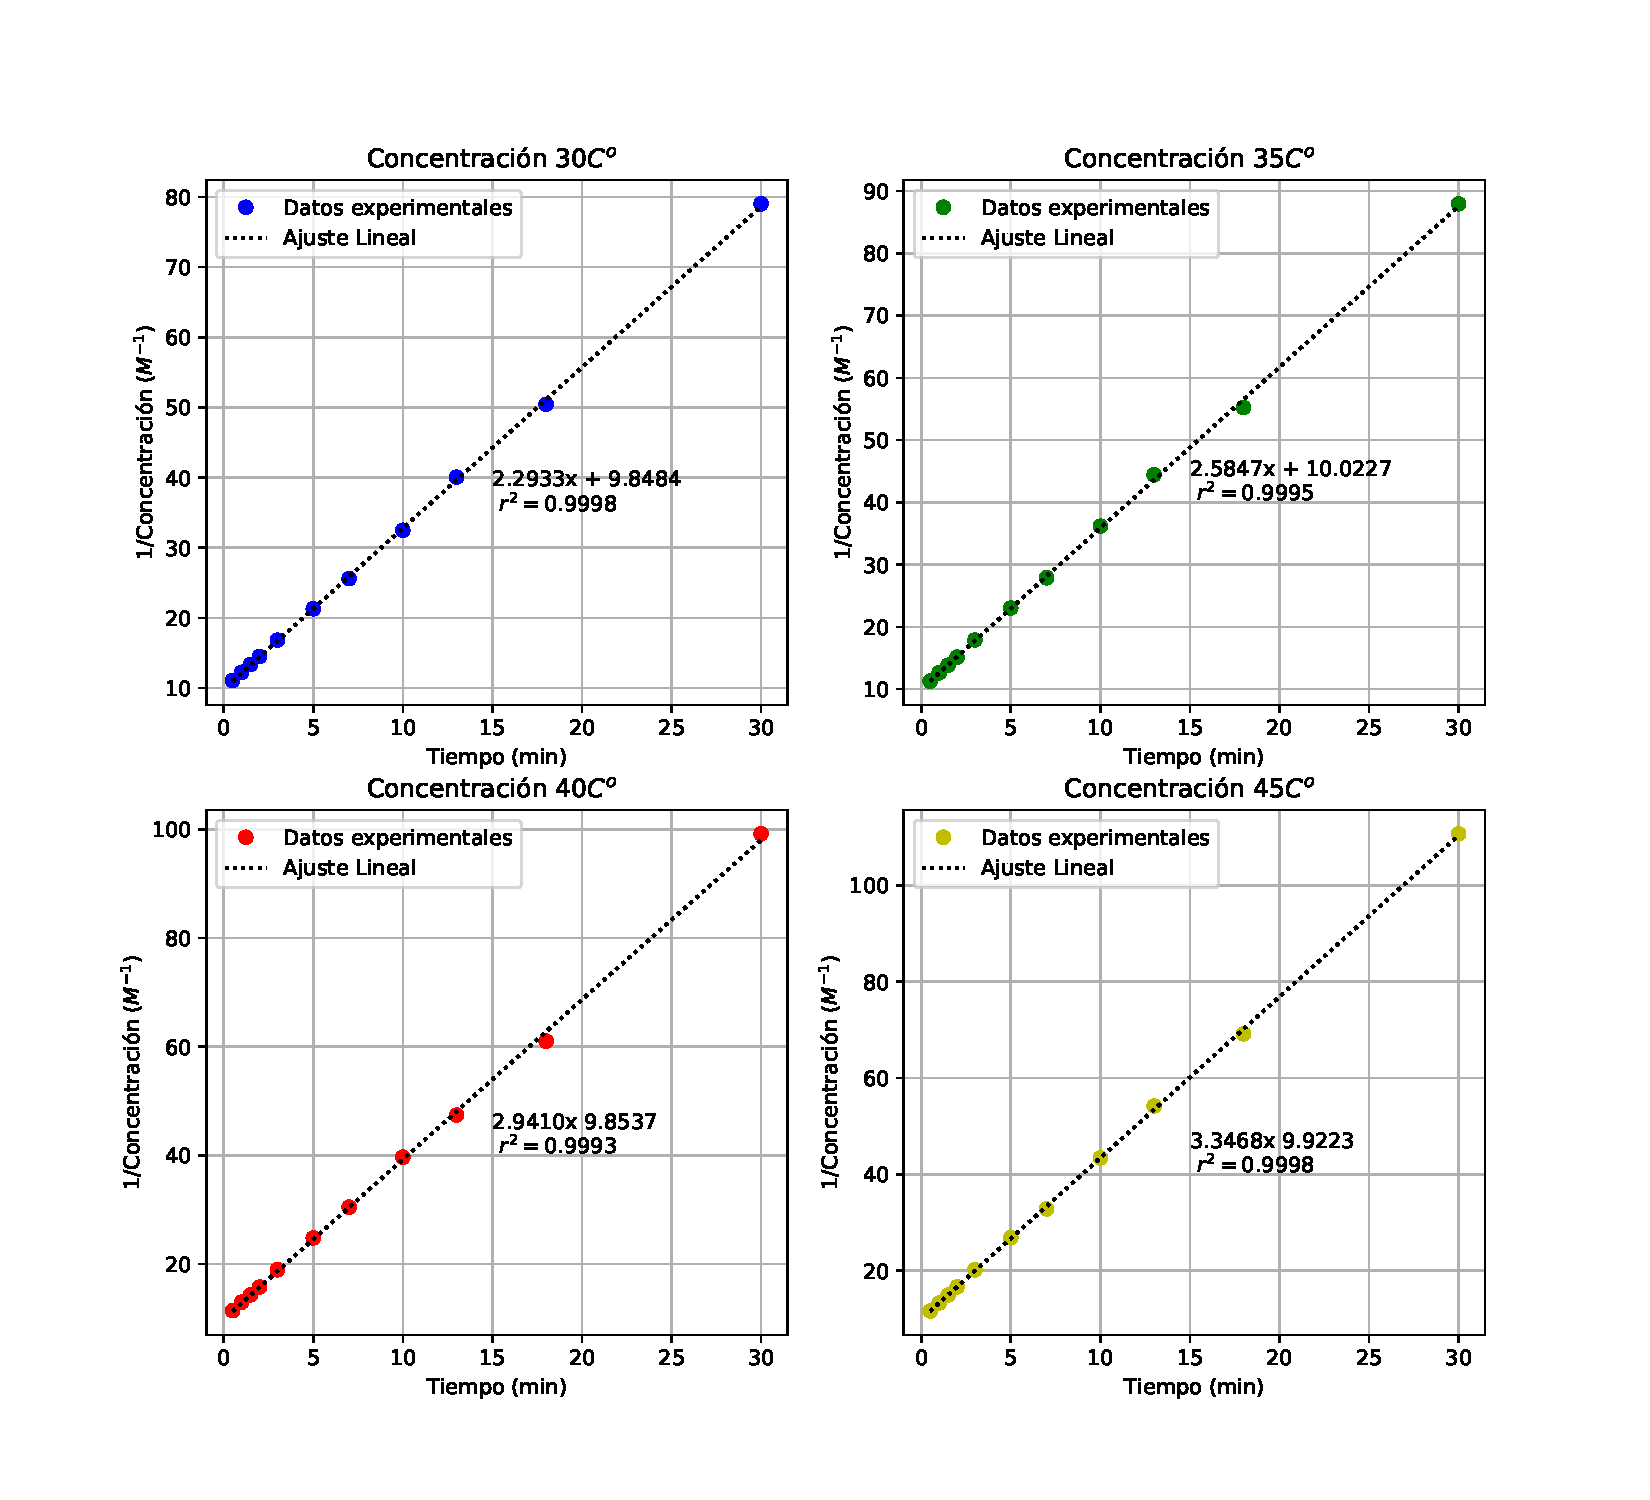
\includegraphics[scale=1]{Figuras/C_45.pdf}
%         \caption{Diagrama de la pr\'{a}ctica}
%\end{figure}

%\end{commet}









\end{document}
